\documentclass{article} % For LaTeX2e
\usepackage{iclr2022_conference,times}
% Optional math commands from https://github.com/goodfeli/dlbook_notation.
\input{math_commands.tex}

%######## APS360: Uncomment your submission name
%\newcommand{\apsname}{Project Proposal}
\newcommand{\apsname}{Progress Report}
%\newcommand{\apsname}{Final Report}

%######## APS360: Put your Group Number here
\newcommand{\gpnumber}{42}

\usepackage{hyperref}
\usepackage{url}
\usepackage{graphicx}

%######## APS360: Put your project Title here
\title{PROJECT TITLE}


%######## APS360: Put your names, student IDs and Emails here
\author{Vedansh Mehta  \\
Student\# 1008973577 \\
\texttt{vedansh.mehta@mail.utoronto.ca} \\
\And
Nathan Shreve  \\
Student\# 1004404487 \\
\texttt{n.shreve@mail.utoronto.ca} \\
\AND
William Wen  \\
Student\# 1007956650 \\
\texttt{jwilliam.wen@mail.utoronto.ca} \\
\And
Paul Zhao \\
Student\# 1009052276 \\
\texttt{paul.zhao@mail.utoronto.ca} \\
\AND
}

% The \author macro works with any number of authors. There are two commands
% used to separate the names and addresses of multiple authors: \And and \AND.
%
% Using \And between authors leaves it to \LaTeX{} to determine where to break
% the lines. Using \AND forces a linebreak at that point. So, if \LaTeX{}
% puts 3 of 4 authors names on the first line, and the last on the second
% line, try using \AND instead of \And before the third author name.

\newcommand{\fix}{\marginpar{FIX}}
\newcommand{\new}{\marginpar{NEW}}

\iclrfinalcopy 
%######## APS360: Document starts here
\begin{document}


\maketitle

\begin{abstract}
    % ABSTRACT HERE
    %######## APS360: Do not change the next line. This shows your Main body page count.
    ----Total Pages: \pageref{last_page}
\end{abstract}



\section{Project Description}

% PROJECT DESCRIPTION SECTION HERE

\section{Individual Contributions and Responsibilities}

% CONTRIBUTIONS AND RESPONSIBILITIES SECTION HERE

\section{Notable Contributions}
\subsection{Data Processing}

For data processing, we implemented a two-step approach. The first step splits the data and saves it into properly structured folders for easy extraction later. The second step involves using a data loader to perform random resizing, converting to tensors, and normalizing to mean 0 and standard deviation 1. Separating these steps allows for easy customization of data transformations for different architectures.

\subsubsection{Source of Dataset}
The dataset for our project, named the \textbf{Chameleon Dataset}, was obtained from the paper \emph{A Sanity Check for AI-Generated Image Detection}, published at ICLR 2025 \citep{yan2024sanity}. We selected this dataset for two main reasons:

\begin{itemize}
    \item It contains a balanced collection of real and AI-generated images across multiple categories, including humans, animals, objects, and scenes.
    \item Unlike datasets such as AIGCDDetect and GenImage (Figure \ref{Chameleon}), which contain raw AI-generated images with visible artifacts, the AI-generated images in the Chameleon dataset are carefully refined by photographers and AI artists. These high-quality images have been shown to fool nine off-the-shelf AI-generated image detectors \citep{yan2024sanity}.
\end{itemize}

\begin{figure}[h]
    \centering
    \includegraphics[width=1\textwidth]{figs/Chameleon.jpg}
    \caption{Comparison between AIGCDDetect (a) and GenImage (b) with Chameleon Dataset(c) \citep{yan2024sanity}.}
    \label{fig:Chameleon}
\end{figure}

Given our goal of detecting general AI-generated images, training our model on this challenging dataset should enable it to generalize well to common tasks, such as differentiating raw AI-generated images.

\subsubsection{Data Splitting}
Our model follows a two-step architecture:
\begin{enumerate}
    \item \textbf{Step 1:} Training a Convolutional AutoEncoder (CAE) using only real images.
    \item \textbf{Step 2:} Training a classifier using both real and fake images.
\end{enumerate}

To prepare our dataset for this architecture, we implemented the following steps:
\begin{enumerate}
    \item Load the Chameleon dataset (ZIP file) from Google Drive.
    \item Unzip the file and extract image paths from the \texttt{01\_real} and \texttt{02\_fake} folders.
    \item Shuffle the images to ensure randomness in splitting.
    \item Identify the total number of real images: 14,863.
    \item Split the real images into two halves:
    \begin{itemize}
        \item One half is used for CAE training.
        \item The other half is paired with fake images for classifier training.
    \end{itemize}
    \item Randomly select the same number of fake images (14,863) to ensure a balanced dataset.
    \item Split the dataset into train, validation, and test sets with a 75-20-5 ratio.
    \item Store the images in structured directories on a shared Google Drive.
\end{enumerate}

We have written helper functions to automate these steps, making the process easily reproducible and applicable to other datasets if additional data is required.

Figure \ref{fig:cleaned_statistic} summarizes the number of images in each split:
\begin{figure}[h]
    \centering
    \includegraphics[width=0.6\textwidth]{figs/cleaned_statistic.png}
    \caption{Statistics from the processed dataset.}
    \label{fig:cleaned_statistic}
\end{figure}

\subsubsection{Data Processing and Augmentation}
The processing step occurs after loading the data using a data loader. The current preprocessing pipeline involves randomly resizing images to 256x256 through cropping to fit our architecture, converting them to tensors, and normalizing them with a mean of (0.5, 0.5, 0.5) and a standard deviation of (0.5, 0.5, 0.5). 

No data augmentation has been applied yet. However, we are considering methods such as flipping, and color jittering, which may be implemented depending on the training results.

We deliberately chose not to perform compression artifact removal, as we believe that compression artifacts might serve as distinguishing features for AI-generated images. However, we have considered tools for compression defect removal, such as Hi-IR \citep{li2024hierarchicalinformationflowgeneralized}, given that our dataset images are in JPEG format and may be subject to compression loss.

Examples of processed images:
\begin{figure}[h]
    \centering
    \includegraphics[width=1\textwidth]{figs/data_examples.png}
    \caption{Examples of cleaned samples from the dataset.}
    \label{fig:cleaned_sample}
\end{figure}

\subsubsection{Future Test Set}
While we have set aside 5\% of the dataset for testing on each step, we still need an external test set to evaluate the model on never-before-seen data as a final step. To achieve this, we plan to:

\begin{itemize}
    \item Collect 100 real-world images from personal sources, covering humans, animals, objects, and scenes.
    \item Generate 100 AI-generated images using state-of-the-art generators such as DALL-E, MidJourney, and Stable Diffusion.
\end{itemize}

\subsubsection{Challenges Faced}
One of the main challenges we encountered was uploading the Chameleon Dataset, which is approximately 2.7 GB in size. Initially, this process was time-consuming when using a direct upload to Google Drive. To address this, we opted to upload the dataset as a ZIP file and extract it directly within PyTorch, significantly reducing transfer times.

Another challenge was the complexity of our data splitting process. Given that our project requires separate data allocations for the Convolutional AutoEncoder and the classifier, a standard split was not sufficient. We resolved this by implementing helper functions that automate the structured splitting and ensure reproducibility across different datasets

\begin{figure}[h]
    \centering
    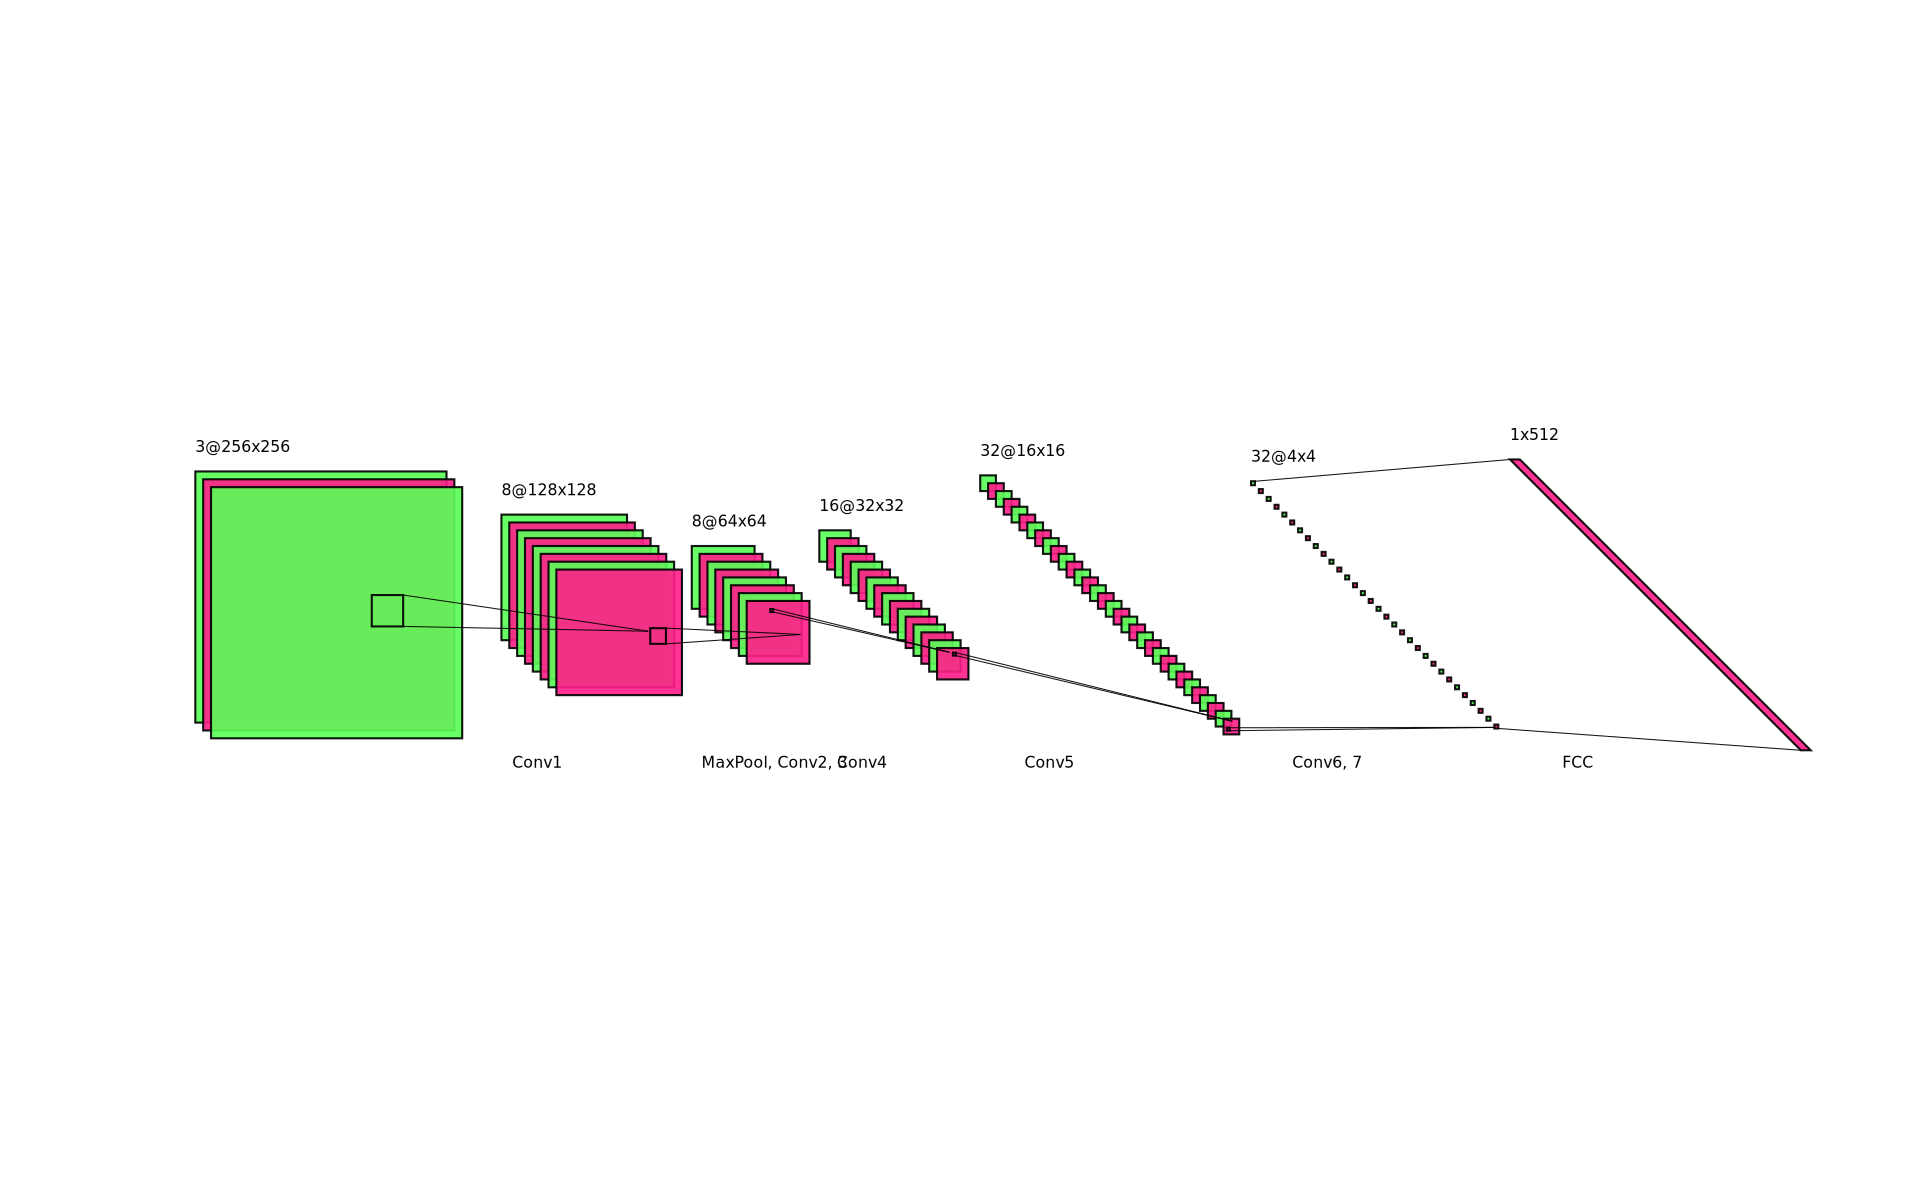
\includegraphics[width=1\textwidth]{figs/baseline.png}
    \caption{Our baseline model and step 2 classifier}
    \label{fig: baseline}
\end{figure}

\begin{figure}[h]
    \centering
    \includegraphics[width=1\textwidth]{figs/cae_illustration.png}
    \caption{Illustraion of Convolution Autoencoder}
    \label{fig:cae}
\end{figure}

\subsection{Baseline Model}

As outlined in the Project Proposal, we wrote a ResNet-inspired CNN inspired by CITE. As detailed in Table \ref{baseline_arch}, it has seven convolutional layers and a total of $1,195,009$ parameters. The hyperparameters we used are those used in CITE, as outlined in our Project Proposal, except for the learning rate and optimizer:
\begin{itemize}
    \item The activation function used was ReLU.
    \item We used a binary cross-entropy loss function.
    \item We used stochastic gradient descent (SGD) with momentum 0.9.
    \item We used a batch size of 64.
    \item We used a learning rate of 0.01.
    \item We trained over ~3000 iterations, which corresponds to 17 epochs.
\end{itemize}

Initially, we had proposed using a step decay learning rate scheduler, but this was outperformed by a constant learning rate. Also, we initially planned to use Adam, but SGD outperformed it.

\begin{table}[t]
    \caption{Baseline model architecture.}
    \label{baseline_arch}
    \begin{center}
        \begin{tabular}{llllll}
            \multicolumn{1}{c}{\bf Layer No.} & \multicolumn{1}{c}{\bf Layer Type} & \multicolumn{1}{c}{\bf Skip Connection From} & \multicolumn{1}{c}{\bf Output Dimensions (C×H×W)}
            \\ \hline \\
            0                                 & Input                              & N/A                                          & 3×256×256                                         \\
            1                                 & Convolutional                      & None                                         & 64×128×128                                        \\
            2                                 & Max pooling                        & None                                         & 64×64×64                                          \\
            3                                 & Batch normalization                & None                                         & 64×64×64                                          \\
            4                                 & Convolutional                      & None                                         & 64×64×64                                          \\
            5                                 & Batch normalization                & None                                         & 64×64×64                                          \\
            6                                 & Convolutional                      & Input to Layer 4                             & 64×64×64                                          \\
            7                                 & Batch normalization                & None                                         & 64×64×64                                          \\
            8                                 & Convolutional                      & None                                         & 128×32×32                                         \\
            9                                 & Batch normalization                & None                                         & 128×32×32                                         \\
            10                                & Convolutional                      & Input to Layer 7                             & 128×32×32                                         \\
            11                                & Batch normalization                & None                                         & 128×32×32                                         \\
            12                                & Convolutional                      & None                                         & 256×16×16                                         \\
            13                                & Batch normalization                & None                                         & 256×16×16                                         \\
            14                                & Convolutional                      & Input to Layer 11                            & 256×16×16                                         \\
            15                                & Average pooling                    & None                                         & 256×4×4                                           \\
            16                                & Batch normalization                & None                                         & 256×4×4 → 4096                                    \\
            17                                & Fully connected                    & None                                         & 1                                                 \\
        \end{tabular}
    \end{center}
\end{table}

We observed that, across various hyperparameter combinations, validation curves were quite jagged, though they declined with the training curve (see Figure \ref{baseline_curves}). The model learns the training data slowly, yet struggles to generalize. This is most likely due to the complex nature of the task, which demands greater parameters and epochs than ours. In our best model we were able to achieve a validation accuracy of 67.0\% and a testing accuracy of 65.6\%. Detailed classification statistics for each split can be seen in Table \ref{baseline_stats}.

\begin{table}[t]
    \caption{Baseline model error statistics; real images are negatives and AI-generated images are positives.}
    \label{baseline_stats}
    \begin{center}
        \begin{tabular}{llllll}
            \multicolumn{1}{c}{\bf Split} & \multicolumn{1}{c}{\bf Loss} & \multicolumn{1}{c}{\bf Accuracy} & \multicolumn{1}{c}{\bf Precision} & \multicolumn{1}{c}{\bf Recall} & \multicolumn{1}{c}{\bf F1 Score}
            \\ \hline \\
            Training                      & 0.303                        & 87.3\%                           & 85.8\%                            & 89.5\%                         & 87.6\%                           \\
            Validation                    & 0.947                        & 67.0\%                           & 66.2\%                            & 69.6\%                         & 67.8\%                           \\
            Testing                       & 0.919                        & 65.6\%                           & 64.7\%                            & 68.5\%                         & 66.6\%                           \\
        \end{tabular}
    \end{center}
\end{table}

\begin{figure}[h]
    \label{baseline_curves}
    \begin{center}
        \includegraphics[scale=0.45]{figs/baseline_error_curves.png}
        \includegraphics[scale=0.45]{figs/baseline_loss_curves.png}
    \end{center}
    \caption{Training/validation error (left) and loss (right) curves for the best baseline model.}
\end{figure}

\subsection{Primary Model}

We outlined a two-step anomaly detection approach in our Project Proposal. In the first step, we trained a convolutional autoencoder (CAE) to encode and decode real images only. In the second step, we feed both real and AI-generated images into the CAE, compute pixel-wise loss, and give this loss to a convolutional neural network (CNN) which classifies the image as real or AI-generated. The advantage of this two-step strategy is that the first is zero-shot, and would not require retraining upon the advent of new image synthesis models. However, we have struggled with this approach and propose new ideas in section \ref{next_steps}.

\subsubsection{Convolutional Autoencoder}

The purpose of our CAE is to model real images well, so it was trained only on real images. It uses up to seven convolutional layers for the encoder and decoder each, with up to $1,970,755$ parameters. We experimented with 30 different combinations of the following hyperparameters to arrive at our best model so far:

\begin{itemize}
    \item Activation function (LeakyReLU, ReLU, TRec CITE)
    \item Use of kernel bias
    \item Number of encoder/decoder convolutional layers
    \item Use of He weight initialization
    \item Batch size
    \item Learning rate
    \item Optimizer (Adam, SGD)
    \item Loss function (mean squared error (MSE), L1 loss, Huber loss, perceptual loss using VGG18 CITE)
\end{itemize}

Below are a number of the challenges we encountered in training the net and how we overcame them.

\begin{itemize}
    \item[1.] During early experimentation, we usually used six layers. We noticed early overfitting in a number of cases using SGD (within the first one to four epochs), and hypothesized that the net was too easily memorizing our data since there were too few parameters. We were able to help this issue by using seven convolutional layers instead of six. However, this resulted in higher overall error even over many epochs, since we had not only increased the number of parameters but also reduced the bottleneck size of our autoencoder.
    \item[2.] Early on, we used a learning rate of 0.01. We also observed that the Adam optimizer was extremely ineffective and could not generalize: validation curves oscillated without decreasing. We then attempted to use a learning rate of 0.0001, and the validation loss greatly decreased in early epochs before overfitting.
\end{itemize}

Our best model used LeakyReLU, no weight initialization, a batch size of 64, a learning rate of $0.0001$, the Adam optimizer with weight decay of $0.01$, and MSE loss. We also used six encoder/decoder layers, which correspond to a compression ratio of 48. Though this model overfit early during training (see Figure \ref{cae_curves}), we were not able to achieve a lower validation loss before overfitting occurred when using lower learning rates. This model achieves a validation MSE of $8.4\%$ and a test MSE of $8.3\%$, which correspond to about $14.4\%$ absolute error per pixel.

\begin{figure}[h]
    \label{cae_curves}
    \begin{center}
        \includegraphics[width=0.6\textwidth]{figs/cae_error_curves.png}
    \end{center}
    \caption{Training/validation error curves for the best convolutional autoencoder.}
\end{figure}

As mentioned earlier, we want the CAE to model real images well and to model AI-generated images badly. Therefore, we also evaluated this model on a separate test set containing both real and AI-generated images with the expectation that the error would be much higher. However, it was also $8.3\%$, suggesting that our CAE has not learned the characteristics that comprise real images, but rather the semantic content of our dataset and possibly patterns produced by the images' compression. The output of the CAE for one real and one AI-generated image is shown in Figure \ref{reconstructions}. We can see that it reconstructs both with an equal lack of detail, suggesting it has not really learned a good representation of real images. This may due to our compression ratio being too high, or, because the differences between the two classes may be too subtle for our current architecture, like with our baseline model.

\begin{figure}[h]
    \label{reconstructions}
    \begin{center}
        \includegraphics[scale=0.45]{figs/real_face_orig.png}
        \includegraphics[scale=0.45]{figs/real_face_recon.png}
        \includegraphics[scale=0.45]{figs/fake_face_orig.png}
        \includegraphics[scale=0.45]{figs/fake_face_recon.png}
    \end{center}
    \caption{Best autoencoder's reconstructions of real (top) and AI-generated (bottom) faces.}
\end{figure}

\subsubsection{Classifier}

The input to our classifier is the pixel-wise CAE reconstruction loss at the output of our CAE. We have experimented with a number of reconstruction loss functions, such as MSE, L1 loss, and Huber loss.

This step is still in early development. At the moment, our classifier uses the same architecture as our baseline model, but without skip connections. However, we have not been able to achieve much better than random results (approximately 50\% accuracy). As mentioned earlier, this is most likely because our CAE models real and fake images equally well.

\subsubsection{Next Steps}
\label{next_steps}

Below are a number of new ideas we will implement that address our struggles outlined above. Some of them build on our work so far, and others will take us in new directions. They are ordered based on priority.

\begin{itemize}
    \item[1.] Use transfer learning, such as ResNet or AlexNet: pass our images through a pretrained model, and pass the output either into our autoencoder or directly to a decoder.
    \item[2.] Train the autoencoder and classifier end-to-end, with a much shallower autoencoder. However, this solution is not zero-shot.
    \item[3.] Use transfer learning to classify our images into a small number of classes (around 10), then train an autoencoder for each class. 
    \item[4.] Find new data, in particular images that are uncompressed, to either supplement or supplant our current dataset.
    \item[5.] Continue to experiment with various hyperparameters on our classifier.
    \item[6.] Follow the method outlined in [CITE ZED paper].
\end{itemize}

\label{last_page}

\bibliography{APS360_ref}
\bibliographystyle{iclr2022_conference}

\end{document}
